%%%%%%%%%%%%%%%%%%%%%%%%%%%%%%%%%%%%%%%%%%%%%%%%%%%%%%%
% A template for Wiley article submissions.
% Developed by Overleaf. 
%
% Please note that whilst this template provides a 
% preview of the typeset manuscript for submission, it 
% will not necessarily be the final publication layout.
%
% Usage notes:
% The "blind" option will make anonymous all author, affiliation, correspondence and funding information.
% Use "num-refs" option for numerical citation and references style.
% Use "alpha-refs" option for author-year citation and references style.

\documentclass[alpha-refs]{wiley-article}
% \documentclass[blind,num-refs]{wiley-article}


\usepackage{booktabs} % For formal tables
\usepackage{tikz}
\usepackage{tikz-qtree}
\usetikzlibrary{trees} % this is to allow the fork right path
\usepackage{soul}
\usepackage{multirow}
\usepackage{array}
\usepackage[skip=5pt]{caption}

\newcolumntype{L}[1]{>{\raggedright\let\newline\\\arraybackslash\hspace{0pt}}m{#1}}
\newcolumntype{C}[1]{>{\centering\let\newline\\\arraybackslash\hspace{0pt}}m{#1}}
\newcolumntype{R}[1]{>{\raggedleft\let\newline\\\arraybackslash\hspace{0pt}}m{#1}}

\graphicspath{ {images/} }

% Add additional packages here if required
\usepackage{siunitx}

% Update article type if known
\papertype{Original Article}
% Include section in journal if known, otherwise delete
\paperfield{Journal Section}

\title{Anticipatory Development Processes for Reducing Total Ownership Costs and Schedules}

% List abbreviations here, if any. Please note that it is preferred that abbreviations be defined at the first instance they appear in the text, rather than creating an abbreviations list.
%\abbrevs{ABC, a black cat; DEF, doesn't ever fret; GHI, goes home immediately.}

% Include full author names and degrees, when required by the journal.
% Use the \authfn to add symbols for additional footnotes and present addresses, if any. Usually start with 1 for notes about author contributions; then continuing with 2 etc if any author has a different present address.
%\author[1\authfn{1}]{Author One PhD}
%\author[2\authfn{1}]{Author A.~Two MD}
%\author[2\authfn{2}]{Author Three PhD}
%\author[2]{Author B.~Four}

\author[1]{Barry Boehm}
\author[1]{Pooyan Behnamghader}

%\contrib[\authfn{1}]{Equally contributing authors.}

% Include full affiliation details for all authors
%\affil[1]{Department, Institution, City, State or Province, Postal Code, Country}
%\affil[2]{Department, Institution, City, State or Province, Postal Code, Country}
\affil[1]{Computer Science Deparment, University of Southern California, Los Angeles, California, 90007, USA}

%\corraddress{Author One PhD, Department, Institution, City, State or Province, Postal Code, Country}
%\corremail{correspondingauthor@email.com}
\corraddress{Barry Boehm, Computer Science Department, University of Southern California, Los Angeles, California, 90007, USA}
\corremail{boehm@usc.edu}

%\presentadd[\authfn{2}]{Department, Institution, City, State or Province, Postal Code, Country}
\presentadd[\authfn{2}]{Department of Computer Science, University of Southern California, Los Angeles, California, 90007, USA}

\fundinginfo{This material is based upon work supported in part by the U.S. Department of Defense through the Systems Engineering Research Center (SERC) under Contract H98230-08-D-0171. SERC is a federally funded University Affiliated Research Center managed by Stevens Institute of Technology. It was also supported by the National Science Foundation grant CMMI-1408909, Developing a Constructive Logic-Based Theory of Value-Based Systems Engineering.}

% Include the name of the author that should appear in the running header
\runningauthor{B. Boehm et al.}

\begin{document}

\maketitle

\begin{abstract}
Many systems and software processes overfocus on getting a project and product from an initial set of requirements to an initial operational capability (IOC).  Examples are most waterfall and V models.  Projects following such processes may pass acceptance tests for functionality and performance, but may leave the product with serious maintainability shortfalls.  Many agile processes focus on users' initial usage priorities, but often make development commitments for earlier needs that are incompatible with achieving later critical needs (e.g., security, safety).  Incremental development process models can do better, but often later increments may find that the earlier increments have not prepared them for ease of modification and repair.  Besides increasing total ownership costs (TOCs), long mean times to repair result in long downtimes, which can be critical to an organization's income and reputation.  Further, many of these shortfalls take the form of Technical Debt (TD), in that the later they are fixed, the more
slow and 
expensive will be the fixes. 
%This is one of the main reasons that organizations spend around 75\% of their software funds on post-delivery maintenance.

This paper summarizes three process frameworks and tools providing more anticipatory ways to improve systems and software maintainability and life-cycle cost-effectiveness.  The first framework is an Opportunity Tree for identifying and anticipating such ways. 
The second framework (SQUAAD) is a toolset for tracking a software project's incremental code commits, and analyzing and visualizing each commit's incremental and cumulative TD.
%, using several sources of TD analysis. 
The third framework is a System and Software Maintenance Readiness Framework (SMRF), that identifies needed software maintenance readiness levels at development decision reviews, similar to the Technology Readiness Levels framework.
%It addresses three components of maintenance readiness: management; personnel; and methods, processes, and tools (MPTs).


% Please include a maximum of seven keywords
\keywords{Software Engineering, Software Maintainability, Software Process, Software Life Cycle Costs, Software Development}
\end{abstract}


\section{Introduction}
\label{sec:introudction}

The inexorable increase in software demand and the pace of changes in software technology, competition, interdependencies, and sources of vulnerability, will seriously strain the capacity of the available software maintenance labor force.

We have been involved in several aspects of analyzing and addressing the root causes of expensive software maintenance.
These include serving on assessments of
exemplary and
problem software projects in government and industry;
evolving and calibrating models for estimating software development and maintenance costs;
leading a multi-year, multi-university US Department of Defense Systems Engineering Research Center to research and develop Systems and Software Qualities Ontology, Tradespace, and Affordability (SQOTA) capabilities;
and researching, developing, and evaluating promising methods, processes, and tools (MPTs) for improving software life cycle productivity and qualities.

We try to quantify such relationships where possible.
For example, the 2015 US General Accountability Office report \cite{dodaro2015government} identified annual US Government Information Technology (IT) expenditures of \$79 billion, of which \$58 billion were in operations and maintenance (O\&M).
Table \ref{tab:pdlcc} provides more detail on fractions of hardware and software costs from the 2008 Redman \cite{redman2008weapon} and  2009 Koskinen \cite{koskinen2009software} studies.


\begin{table}[htbp]
	\centering
	\caption{Percentage of Post-Deployment Life Cycle Cost}
	\resizebox{\columnwidth}{!}{
		
		% Table generated by Excel2LaTeX from sheet 'Sheet1'
		\begin{tabular}{ll}
			\toprule
			\textbf{Hardware (Redman, 2008)} & \textbf{Software (Koskinen, 2009)} \\
			\midrule
			12\% -- Missiles (average) & 75-90\% -- Business, Command-Control \\
			60\% -- Ships (average) & 50-80\% -- Complex cyber-physical systems \\
			78\% -- Aircraft (F-16) & 10-30\% -- Simple embedded software \\
			84\% -- Ground vehicles (Bradley) &  \\
			\bottomrule
		\end{tabular}%		
	}
	\label{tab:pdlcc}
	\vspace{-0.3cm}
\end{table}%

The SQOTA ontology identified Maintainability as not only supporting Affordability in terms of total ownership costs, but also supporting Changeability and Dependability (see Table \ref{tab:SERC_Stakeholder}). Maintainability supports Changeability in terms of rapid adaptability to new opportunities and threats, and also supports Dependability in terms of Availability, in that reducing Mean Time to Repair (MTTR) for a system with a given Reliability in terms of Mean Time Between Failures (MTBF) improves Availability via the equation Availability = MTBF / (MTBF+MTTR) \cite{IIS2:IIS2278}.

Note also that the SQOTA ontology’s definition of the key quality of Resilience or the combination of Dependability and Changeability is consistent with the INCOSE Systems Engineering Handbook’s definition of Resilience or “the ability to prepare and plan for, absorb or mitigate, recover from, or more successfully adapt to actual or potential adverse events,”
\cite{incose2015systems,haimes2012systems}.

Many system development projects strongly focus on creating and evaluation the systems’ Initial Operational Capability (IOC). In doing so, they often miss opportunities to make the system more cost-effectively maintainable. 
More recently, both commercial and defense organizations have found it competitively critical to perform continuous development \& delivery, or DevOps, involving significant changes in preparing for post-IOC evolution, as recommended in \cite{DefenseScienceBoard}.

\begin{table}[htbp]
	\centering
	\caption{Upper Levels of SERC Stakeholder Value-Based System Quality (SQ) Means-Ends Hierarchy \cite{IIS2:IIS2278}}
	\resizebox{\columnwidth}{!}{
		
		% Table generated by Excel2LaTeX from sheet 'StakeHolder'
		\begin{tabular}{ L{2.7cm} | L{9cm}}
			\toprule
			Stakeholder Value-Based SQ Ends & Contributing SQ Means \\
			\midrule
			Mission Effectiveness & Stakeholders-Satisfactory Balance of Physical Capability, Cyber Capability, Human Usability, Speed, Endurability, Maneuverability, Accuracy, Impact, Scalability, Versatility, Interoperability, Domain-Specific Objectives \\
			\midrule
			Life Cycle Efficiency & Development and \textbf{Maintenance Cost}, Duration, Key Personnel, Other Scarce Resources; Manufacturability, Sustainability \\
			\midrule
			Dependability & Reliability, \textbf{Maintainability}, Availability, Survivability, Robustness, Graceful Degradation, Security, Safety \\
			\midrule
			Changeability & \textbf{Maintainability}, Modifiability, Repairability, Adaptability \\
			\midrule
			Composite QAs &  \\
			\midrule
			Affordability & Mission Effectiveness, Life Cycle Efficiency \\
			\midrule
			Resilience & Dependability, Changeability \\
			\bottomrule
		\end{tabular}%
	}
	\label{tab:SERC_Stakeholder}%
	\vspace{-0.3cm}
\end{table}%


Section \ref{sec:opportunity_tree} summarizes the Opportunity Tree of ways to improve systems and software maintainability and life-cycle cost-effectiveness. 
Section \ref{sec:squaad} summarizes the Software Quality Understanding by Analysis of Abundant Data (SQUAAD) toolset for tracking a software project's incremental code commits, and analyzing and visualizing each commit's incremental and cumulative Technical Debt (TD).
Section \ref{sec:smrf} summarizes the Systems and Software Maintenance Readiness Framework (SMRF), that identifies needed maintenance readiness levels, and reflects that many sources of TD are non-technical.
Section \ref{sec:conclusion} summarizes the resulting conclusions.
\section{MAINTAINABILITY OPPORTUNITY TREE}
\label{sec:opportunity_tree}
Figure \ref{fig:opportunity_tree} provides an opportunity tree for Maintainability.   As with our other opportunity trees for reducing Cost, reducing Schedule, and improving Dependability aspects, it provides a checklist for systems engineers and developers to use in improving a system's Maintainability.


\begin{figure}[h]
	\vspace{-0.3cm}
	\centering
	\resizebox{\columnwidth}{!}{
		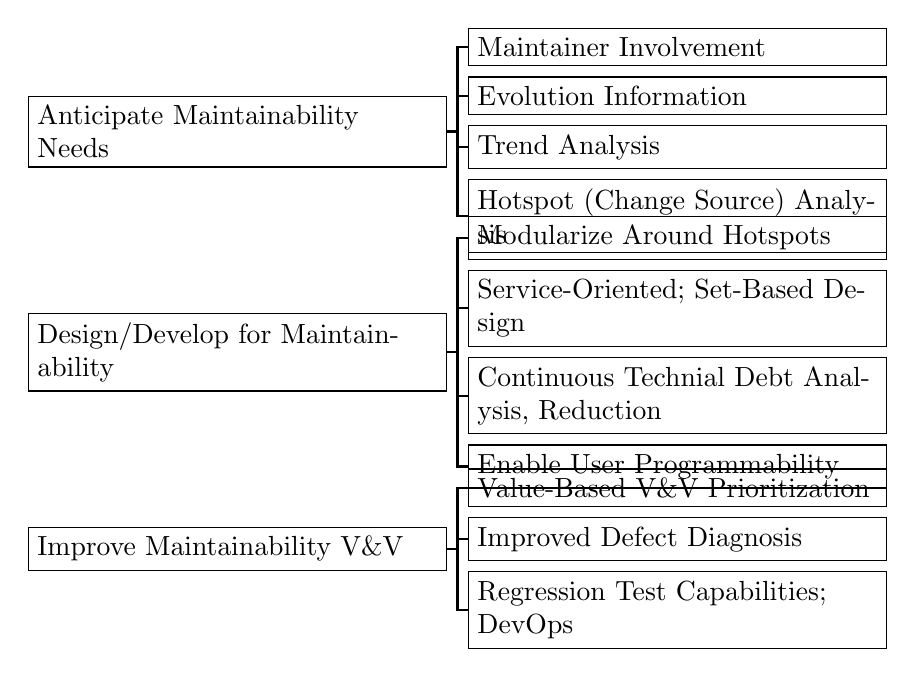
\begin{tikzpicture}[grow'=right,level distance=2.2in,sibling distance=.05in]
		\tikzset{
			edge from parent/.style= 
			{thick, draw, edge from parent fork right},
			every tree node/.style=
			{draw,minimum width=2in,text width=2in,align=left},
		}
		\begin{scope}
		\Tree 
		[.{Anticipate\ Maintainability\ Needs}
		[.{Maintainer\ Involvement} ]
		[.{Evolution\ Information} ]
		[.{Trend\ Analysis} ]
		[.{Hotspot\ (Change\ Source)\ Analysis} ]
		]
		\end{scope}
		\begin{scope}[yshift=-2.8cm]
		\Tree
		[.Design/Develop\ for\ Maintainability
		[.{Modularize\ Around\ Hotspots} ]
		[.{Service-Oriented;\ Set-Based\ Design} ]
		[.{Continuous\ Technial\ Debt\ Analysis,\ Reduction} ]
		[.{Enable\ User\ Programmability} ]
		]
		\end{scope}
		\begin{scope}[yshift=-5.3cm]
		\Tree
		[.Improve\ Maintainability\ V\&V
		[.{Value-Based\ V\&V\ Prioritization} ]
		[.{Improved\ Defect\ Diagnosis} ]
		[.{Regression\ Test\ Capabilities;\ DevOps} ]
		]  
		\end{scope}
		\end{tikzpicture}
	}
	\caption{Maintainability Opportunity Tree}
	\label{fig:opportunity_tree}
\end{figure}



\textbf{Anticipate Maintainability Needs: Maintainer Involvement.}
Lack of maintainer involvement in system and software development often results in key Maintainability enablers being either neglected or implemented in incompatible ways.   It may take some effort to get the maintainers involved, as often they are stuck in a vicious circle and are too busy overcoming the Maintainability shortfalls caused by previous projects lacking maintainer involvement in their definition and development.

\textbf{Evolution Information and Trend Analysis.}
Often, the requirements for a system acquisition are determined by prioritizing the capabilities, and using a Cost As Independent Variable (CAIV) analysis to determine which capabilities fit within the available budget and are to be included in the Request for Proposal (RFP).   This unfortunately throws away valuable below-the-line information on the most likely directions of system evolution, often leading to a brittle point-solution architecture as the chosen solution.
Including the below-the-line capabilities in the RFP as candidate Evolution Capabilities Information, and indicating that it should be considered in preparing the system's life cycle architecture, is more likely to result in reducing operations and maintenance costs.
Trend Analysis is another way to identify likely directions of system evolution.

\textbf{Hotspot (Change Source) Analysis.} Common sources of change include user interface changes, device driver changes, external interface changes, and changes in Non-Developmental Items (NDIs).
Many Commercial-Off-The-Shelf (COTS) NDI products have new releases every 8-12 months, and continue support for only the latest three releases.  In gathering data for a COTS-integration version of the COCOMO cost model, we found one large project entering maintenance with 120 COTS products, 55 of which were no longer supported \cite{Abts00cocots:a}.  Other NDIs are more volatile: for example, Amazon's cloud services are updated every 11 seconds.  Open-source NDIs vary widely on their change frequency.  Systems employing numerous COTS products, and NDIs may therefore have numerous changes, often becoming too expensive to maintain.

\textbf{Design/Develop for Maintainability: Modularization Around Hotspots.} The 1979 Parnas paper, ``Designing Software for Ease of Extension and Contraction,'' \cite{parnas1979designing} and earlier Parnas papers identify this Maintainability strategy.   Common sources of change that have been encapsulated in modules will contain the change effects within the module rather than having them ripple across the other parts of the system.    Using this and related TRW data-driven strategies enabled large projects to perform maintenance changes at lower costs than development changes \cite{royce1998software}.   

\textbf{Service Orientation; Set-Based Design.} Service-oriented loose coupling is a design principle that is applied to the services in order to ensure that the service contract is independent of the underlying service logic and implementation \cite{sundbo2000innovation}. Basically, the concept of loose coupling provided by a Service-Oriented Architecture (SOA) component is that it publishes a contract indicating that if it is furnished with a specified set of inputs, it will produce a specified set of outputs, without otherwise interacting with the user's environment \cite{boehm2008balancing,borges2004delving}.

If a project has a range of choices among services, algorithms, COTS products, etc., it is often better to identify the strongest sets of choices of each and carry them along in a set-based design and to converge on the best choices as sufficient information becomes available 
\cite{bernstein1998design,reinertsten2009principles}.  Set-based design is also valuable if a system is part of one or more systems of independently-evolving systems.

\textbf{Continuous Technical Debt Analysis and Reduction.}  Technical debt refers to delayed technical work or rework that is incurred when shortcuts are taken.  The shortcuts may have good rationales such as the need to meet a market window or to field defenses against cyber or physical attacks.  Or they may result from poor project coordination or sloppy work habits.  Examples are duplicated code or files; unused code; uninitialized variables; and unguarded exceptions.  Either way, the later the debt is paid, the more it will cost, corresponding to interest on a financial debt.

Finding such sources of technical debt via code inspections can be labor-intensive if done for each commit, or delayed if done for each release, although human-assessed indicators of software understandability have been shown to be helpful in estimating maintenance costs \cite{chen2016evaluating}.  Fortunately, tools are becoming available for assessing software technical debt, such as SonarCube, CAST, PMD, and FindBugs.  Section 3 will summarize the Software Quality Understanding by Analysis of Abundant Data (SQUAAD) toolset for tracking a software project's incremental code commits, and for analyzing and visualizing each commit's incremental and cumulative Technical Debt.

\textbf{Enable User Programmability.} In many circumstances, users have found it easier to develop spreadsheet applications for specific needs rather than trying to master and tailor complex general applications to fit their needs.   Many special devices with numerous options (e.g., medical infusion pumps; educational robots) have simple special-purpose languages for specifying the options.  User Programmability may have problems: an IBM study found that 44\% of a large sample of spreadsheet programs had defects that would if exercised have had major negative financial outcomes for the organization.

\textbf{Improve Maintainability V\&V: Value-Based V\&V Prioritization.}  Most V\&V aids, such as automated test case generation, assume that every test case and defect is equally important.  However, in practice, projects find that the value of running the test cases follows a Pareto distribution, in which 20\% of the test cases produce 80\% of the business value.  For example, one company found that one of its 15 customer sets accounted for 50\% of the business value of prompt billing, and 3 of its customer sets accounted for 80\% of the business value \cite{bullock2000calculating}.   A further industrial application increased the business value of testing their annual product release features from 58\% to 91\% \cite{li2012value}.

\textbf {Regression Test Capabilities; DevOps.}
Amazon's DevOps ability to reliably upgrade its huge variety of services every 11 seconds implies a remarkable ability to perform regression testing of each release's changes.  Providing similarly reliable, rapid large-scale DevOps upgrades will require similar rapid regression testing upgrades.  Software maintenance organizations expected to carry on similar DevOps capabilities would need similar rapid regression testing capabilities, along with further Testability enablers of having and evolving cost-effective test drivers, test oracles, test data management capabilities, and diagnostic capabilities.   






\section{Software Quality Understanding by Analysis of Abundant Data (SQUAAD) Toolset}
\label{sec:squaad}

Software developers can prevent failures and disasters and reduce total ownership costs by putting more emphasis on improving software maintainability in their software development process.
One way to improve software maintainability is to produce clean code while changing the software and to continuously assess and monitor code quality while the software is evolving \citep {mexim2015introduction}.

Prior research has been focusing on the analysis of official releases of software to understand how its code quality evolves \citep{PINTO201559,tu2000evolution,ganpati2012comparative,d2008analysing,le2015empirical}.
This approach gives an insight on change in code quality over the major milestones of software development, rather than how code quality evolves during software development process. 
For example, a developer may unknowingly increase the amount of Technical Debt (TD) over a few commits. If that debt is not addressed quickly, it can impose extra cost.
It gets even worse, if they leave the team without paying that debt.
In another example, a developer may simply commit broken code to the repository.
This will break the code for other contributors and slows down the development.
It also causes the unavailability of byte-code for that commit in a post-development analysis.
Since software developers do not ship uncompilable code in official releases, this detail may not be revealed in that coarse-grained analysis. 

Our approach to understand software quality evolution is not limited to study the official releases but to take a step further by analyzing the state of the software after each commit.
For example, our study on the evolution history of  68 open-source software systems shows from one release to the next one, software contains fewer lines of code, classes, code smells, and security vulnerabilities in 8\%, 4\%, 14\%, and 6\% of times.
However, from one revision (produced by a commit) to the next one, these ratios are 18\%($\uparrow$), 3\%($\downarrow$), 17\%($\uparrow$), and 2\%($\downarrow$).
%Analyzing the impact of each commit on software quality can reveal a wealth of information because it holds details of every stage in the software evolution, such as the time of each change and who made the change.
Analyzing the impact of each commit on software quality can reveal a wealth of information because commits carry fine-grained data on every stage of software evolution, such as the author, the time, and the intent (i.e., commit message) of change.


Over the past couple of years, multiple tools and techniques are introduced to study software evolution by commit-level \citep{Tufano2017TSE,Dyer2015TOSEM,diamantopoulos2016qualboa,Tiwari2017msr,PINTO201559,gousios2014lean,Rozenberg2016MSR,Kaur2018,Sokol2013SCAM,Trautsch2017,Trautsch:2016:APE:2901739.2901753}.
Some of them do not run analysis on source code \citep{gousios2014lean,Rozenberg2016MSR}. 
Some of them are designed and implemented to run source code analysis sequentially \citep{Tufano2017TSE,Sokol2013SCAM}.
Consequently, the execution of the study requires strong on-premise resource and takes multiple weeks \citep{Tufano2017TSE}.
There are some mining techniques designed to scale by running static analysis on different revisions of each file in parallel \citep{Dyer2015TOSEM,AlexandruSANER2017,Trautsch2017}.
These techniques are extremely efficient in generating an Abstract Syntax Tree (AST) \citep{AlexandruSANER2017,Dyer2015TOSEM} and calculating file-based quality metrics, such as size, cohesion, and complexity \citep{Trautsch2017}.
They can also aggregate the result of individual files analysis to evaluate the quality of a project.
However, this approach for achieving scale and avoiding redundancy is not suitable to understand software quality evolution by program analysis techniques that
\begin{itemize}
	\item analyze a \textbf{module} considering all of its source code entities and their \textbf{relationship}.
	For example, architecture recovery techniques generate clusters of source code entities by analyzing semantic and/or structure relationships between them \citep{garcia2013comparative,Tzerpos:2000:AAC:832307.837118}.
	It does not suffice to separately analyze the changed files and aggregate the results to recover the architecture of a new revision.
	%	The artifacts generated by these techniques (clusters of entities) associate 
	\item require \textbf{bytecode}.
	Some static and dynamic program analysis techniques depend on the availability of the compiled version (e.g., FindBugs \citep{4602670} and test-coverage \citep{Malaiya2002ieee}). 
	A commit may change the version of a dependency. 
	The new dependency is available and the build configuration (e.g., \textit{build.gradle}) is syntactically correct.
	However, the new revisions do not compile as the dependency is not backward compatible \citep{Behnamghader2017qrs}.
	A recent study \citep{AlexandruSANER2017} declares the unavailability of the compiled versions as the main unresolved source for the manual effort in software evolution analysis.
\end{itemize}

In addition, some tools rely on a complex \textbf{environment} to run.
This includes dynamic techniques that need an execution environment and static techniques with specific requirements.
For example, SonarQube \citep{campbellsonarqube} requires deploying its own analysis server, generating a configuration file for each revision, executing the analysis, and fetching the results using SonarQube Api.
%There is also a relative scarcity of commit-level empirical study on using complex program analysis techniques (e.g., building the software, running FindBugs on bytecodes, or running architecture recovery) on different modules, COTS tools with complex environments (e.g., SonarQube), and dynamic analysis techniques (e.g., rendering webpages or test-coverage).
%There is also not much work on a multi-perspective analysis and visualization of software quality evolution from a module/system perspective.

We took steps toward addressing that scarcity by developing Software Quality Understanding by Analysis of Abundant Data (SQUAAD) \citep{cser2018behnamghader}, a comprehensive framework including a cloud-based automated infrastructure accompanied by a data analytics toolset and web interfaces.
%XXX In this paper, we introduce Software Quality Understanding by Analysis of Abundant Data \textbf{(SQUAAD)}, a comprehensive framework including a cloud-based automated infrastructure accompanied by a data analytics and visualization tool-set.
%Our integrated tool-based approach has been documented in multiple research publications empowering their empirical studies \citep{le2015empirical,mahajan2016using,Behnamghader2017,10.1007/978-3-319-62217-0_9}.
%Our approach to conduct large-scale replicable empirical studies on software evolution has been to capitalize on cloud services to full maintainability and technical debt commit histories of large families of open-source software systems available through GitHub.
Our multi-perspective software quality evolution approach assesses
%code and architectural changes. 
%It addresses 
%multiple 
different quality attributes such as software size, code quality, and security.
It utilizes complex program analysis techniques (e.g., byte-code analysis using FindBugs and architecture recovery using ACDC), COTS tools with complex environments (e.g., SonarQube), and dynamic analysis (e.g., unit-test pass-rate).
It enables analysis of the conflicts and synergies between different quality attributes and the difference between developers in terms of their impact on software quality.
Our integrated tool-based approach has been documented in multiple research publications \citep{cser2018behnamghader,Behnamghader2018esem,Behnamghader2017qrs,Behnamghader2017,Alfayez2017stc, Alfayez2018TechDebt} empowering their empirical studies and is used by a major governmental entity.


%Our approach to conduct large-scale replicable empirical studies on software evolution has been to capitalize on cloud services to analyze full maintainability and technical debt commit histories of large families of open-source software systems available through GitHub. SQUAAD automatically
%1)	retrieves a subject system's meta-data (e.g., number of contributors) as well as its commit history from GitHub.
%2)	distributes hundreds of revisions (i.e. official releases and/or revisions created by commits) on multiple cloud instances.
%3)	compiles each revision and runs static/dynamic programming analysis techniques.
%4)	collects and parses the artifacts generated by programming analysis techniques to extract quality attributes.
%5)	runs various statistical analysis on software quality evolution.

SQUAAD is designed to target a module, compile its distinct revisions, and run static/dynamic analysis on it.
Before conducting a large-scale analysis, SQUAAD runs a light-weight mining task on the software's Git repository to determine which commit changes a module (impactful commits \citep{Behnamghader2017qrs}) and the evolutionary relationship between those commits \citep{Behnamghader2018esem}.
Then it automatically
% to automatically 1) retrieve a subject system's meta-data (e.g., number of contributors) as well as its commit history (i.e., Git repository), 2) distribute 
1) distributes hundreds of revisions on multiple cloud instances,
2) compiles each revision using default and/or user defined configurations,
3) provisions the environment and runs static/dynamic programming analysis techniques on each revision,
4) collects the generated artifacts,
5) either parses them to extract quality attributes or compares them to each other to calculate the difference (e.g., by architectural distance metrics), and
% and store them in a relational database,
6) runs various statistical analysis on software quality evolution.

The entire analysis workflow is automated. As soon as the framework is configured for a subject system, we can run the represented analysis on that system and study its evolution.
This full automation makes analysis conducted by SQUAAD replicable and addresses a major threat (i.e., not being replicable) to the external validity of repository mining studies \citep{Trautsch:2016:APE:2901739.2901753}.
We have also developed web interfaces to illustrate the evolution of different quality attributes and the impact of each developer on software quality.

%We assessed the generalizability of my current lead-author paper results by extending the dataset used in those studies either in terms of number of subject systems and organizations, or conducting commit-level analysis instead of release-level.

For example,
one of our recent maintainability trends analysis \citep{Behnamghader2017qrs} involves a total of 19,580 examined revisions from 38 Apache-family systems across a timespan from January 2002 through March 2017, comprising 586 MSLOC.
In this analysis, to obtain software quality, we used three widely-used open-source static analysis tools: FindBugs, PMD, and SonarQube.
We selected a subset of quality attributes related to size (basic), code quality, and security.
We found that on average, 2\% of impactful commits break the compilation.
We qualitatively investigated when, how, and why developers break the compilation and introduced a guideline for preventing developers from committing uncompilable code.
%Our results suggest that the impactful commits have different impact on the software quality metrics.
We found that different quality attributes may change even if the size (i.e., code count) of the software does not change.
We calculated the probability for a metric to change while another one is constant based on the collected data.
%Our results also show that although the security metrics change less frequently, it is crucial to utilize them as they can reveal the introduction of different kinds of security problems.
Our result showed that employing multiple security metrics together can reveal points where security problems are introduced.

%In a follow up work , we extended our original dataset to include revisions committed in 2017/18 of those 38 Apache systems, as well as 30 new open-source systems from Google and Netflix, comprising a total of 37838 distinct revisions and more than 1.5 billion lines of code.
In a follow-up study \citep{Behnamghader2018esem}, we extended our original dataset to include 30 new subject systems from Google and Netflix, as well as revisions committed in 2017 and 2018 of 38 Apache systems of the original dataset.
The extended dataset comprises more than 37k analyzed distinct software revisions and more than 1.5 billion lines of code.
We replicated the analysis mentioned above on the new dataset and extended it to reach the maximum commit compilability (97.7\% for Apache, 99.0\% for Google, and 93.9\% for Netflix) and identify all uncompilable commits that are caused by a developer's fault.
We quantitatively analyzed the reasons for introducing compile errors and proposed a model to detect the uncompilable commits in a post-development analysis based on the meta-date of the commits (i.e., time, message, and committer) and without considering code artifacts.
Then we analyzed all compilable commits to understand the difference between affiliated and external developers of each organization in terms of impacting different quality attributes. 
For example, our analysis shows that although there is no difference between affiliated and external developers in terms of changing the size of the software, external developers of Netflix and affiliated developers of Google have higher ratio of compilable commits.

Tools such as SQUAAD can enable organizations to continuously monitor their sources of TD and remove them quickly during development, rather than pay for them with interest during maintenance. We are creating versions for some government support organizations to aid in their monitoring and prioritization of TD and its removal. 

%XXX Focusing on a module helps better understanding of heterogeneous projects that are developed in different programming languages and/or by different development teams.
%For example Apache Avro\footnote{https://github.com/apache/avro} is implemented in more than 10 programing languages in the same repository.
%Instead of evaluating the whole project, we can focus on its Java implementation by targeting the ``lang/java'' module. 
%This also helps analyzing heterogeneous projects even if the utilized program analysis technique does not support all languages.
%In another example, Apache Parquet-MR\footnote{https://github.com/apache/parquet-mr} contains different Java sub-projects.
%Each sub-project has its own set of developers and reviewers.
%Instead of focusing on the whole project, we can focus on each sub-project to evaluate the performance of each team.
%
%In our large-scale studies on software quality evolution by commit-level, we have identified multiple benefits for focusing on modules:
%\begin{enumerate}
%	\item It provides a more \textbf{accurate} analysis by ignoring irrelevant changes.
%	Apache Santuario \footnote{https://github.com/apache/santuario-java} provides implementation of primary security standards for XML.
%	Its core module (``src/main'') is accompanied by a large number of tests (``src/test'') comprising 30\% of all source files.
%	Consequently, 34\% of commits do not change any code in the core module.
%	Mining the whole repository and including those commits may causes inaccuracy when analyzing the frequency of change in a quality metric.
%	For example, in a study of architectural evolution, introduction of a test case is not necessarily an architectural change.
%	However an automated recovery technique may consider it as a change since a new entity is added.
%	\item It provides a more \textbf{complete} view of evolution for some commit-level mining tasks.
%	In several instances, we have observed that a commit introduces a compilation error in one module and causes the whole software to be uncompilable over a period; however, other modules are compilable and are evolving over that period.
%	For example, in Netflix-Spectator\footnote{https://github.com/netflix/spectator} commit fbeb719, a compile error in a unit test breaks the compilability the software.
%	This causes the unavailability of bytecode over a period which results in missing data points and an incomplete analysis of the software evolution.
%	After focusing on the core module and skipping tests we reached a 100\% compilability and obtained a full view of the evolution of the core module.
%	%	Compilation is necessary if the analysis depends on the availability of byte-code.
%	\item It reduces the \textbf{cost} and \textbf{complexity} of the mining task.
%	Apache Tiles \footnote{https://github.com/apache/tiles} is a templating framework for user interface development.
%	It is designed to be integrated with a variety of other systems.
%	Its core module is accompanied with multiple smaller components (e.g., sdk, agents, and plugins). 
%	Although majority (70\%) of developers change the core module at least once, only 24\% of commits change code in that module.
%	Instead of analyzing all commits to understand the quality (e.g., compilability, test coverage, technical debt, security, etc.) of the core module, we can focus on that smaller subset.
%	\item It helps better understanding of heterogeneous projects that are developed by \textbf{different development teams}.
%	Apache Parquet-MR\footnote{https://github.com/apache/parquet-mr} contains different sub-projects in the same repository.
%	Each sub-project has its own set of developers and reviewers.
%	%	Consequently, only 34\% developers change the core sub-project at least once over the whole development history.
%	Instead of focusing on the whole project, we can focus on each sub-project to evaluate the performance of each team.
%	\item It helps better understanding of \textbf{multi-language} projects.
%	%Some repository mining techniques simply skip a repository if their programming analysis techniques do not support all utilized programming languages \citep{dyer2013boa,Dyer2015TOSEM}.
%	Apache Avro\footnote{https://github.com/apache/avro} is implemented in 10 programming languages in the same repository.
%	Instead of analyzing the whole project and dealing with the issues of analyzing multi-language projects \citep{AlexandruSANER2017,Arbuckle:2011:MMS:2024445.2024461}, we can run analysis on each modules (e.g., ``lang/java'', ``lang/c++'') individually by a proper program analysis technique.
%	Some mining repository techniques only support one programming language \citep{Dyer2015TOSEM} or limit their mining task to one language per project \citep{Trautsch:2016:APE:2901739.2901753,Trautsch2017}.
%	\begin{figure} [h]
%		\centering
%%		\includegraphics[width=\columnwidth]{accumulo_all}
%%		\includegraphics[width=\columnwidth]{accumulo_impactfuls}
%		\caption{The evolution of unused code blocks in the core module of Apache Accumulo using two sets of commits: 1) all 8605 commits (top) and 2) 2010 commits that change the core module (bottom).}
%		\label{fig:accumulo}
%		%	\vspace{-0.5cm}
%	\end{figure}
%	\item It improves the \textbf{understandability} of data visualization when thousands of data points are depicted.
%	Apache Accumulo \footnote{https://github.com/apache/accumulo} is a distributed data storage framework.
%	Over a period of 5 years (10/2011 to 11/2016) 105 developers contribute 8605 commits to its repository.
%	Only 2010 commits by 76 developers change accumulo's core module.
%	Figure \ref{fig:accumulo} shows the evolution of the number of unused code blocks in the core module using all commits (top) and only the ones that change the core module (bottom) over that period.
%	Both graphs show the same evolutionary trend, but the top one contains 6595 (3.3x) more data points that are not relevant to changes in the core module.
%	
%	\item It facilitates \textbf{manual inspection} of individual data points which is a labor intensive task.
%	In Apache CXF-Fediz\footnote{https://github.com/apache/cxf-fediz}, commit b06255a changes the core module and uses a new interface, which causes a compile error.
%	The error is fixed in the next commit changing the core module (44d7340) which is a small commit that comments out the line containing the error and says ``Switching to WSS4J 2.0.0-rc1 + commenting some stuff as a result''.
%	There are four other commits changing code in other modules between these two commits.
%	Instead of manually inspecting all 6 commits to understand why the repository is uncompilable, we can analyze those two commits that change the core module.
%	%	Focusing on the core module makes the inspection more efficient. 
%\end{enumerate}
\section{ADDRESSING NON-TECHNICAL SOURCES OF TECHNICAL DEBT}
\label{sec:smrf}

Our multi-year, multi-university US DoD Systems Engineering Research Center (SERC) System Qualities Ontology, Tradespace, and Affordability project has held and participated in several industry-government workshops to clarify the relations among their various systems and software quality attributes.  These have led to the stakeholder value-based, means-ends ontology structure shown in Table \ref{tab:SERC_Stakeholder}, which highlights Maintainability as a key Means to three of the four stakeholder-value Ends categories [35].
The workshops also confirmed the key contribution of Technical Debt to systems and software maintenance costs, and identified that there were a number of non-technical sources of TD, to be summarized in section \ref{subsec:topten}, and addressed via the Systems and Software Maintainability Readiness Framework (SMRF) presented in section \ref{subsec:smrf}.


\subsection{Top-10 List of Major Non-Technical Sources of Technical Debt}
\label{subsec:topten}

The inexorable increase in software demand and the pace of changes in software technology, competition, interdependencies, and sources of vulnerability, will seriously strain the capacity of the available software maintenance labor force.
Recently, a US industry-government workshop was held to address this challenge and what to do about it.
A good deal of the discussion was focused on the high cost of software technical debt \cite{6336722}, and on ways to identify it and reduce it more quickly.
During the discussions, several observations were made that a good many sources of technical debt are non-technical, and that addressing these would likely be cost-effective.
In response, a portion of the workshop was devoted to identifying and prioritizing these non-technical sources of technical debt.

The working group addressing the non-technical sources of technical debt identified 17 non-trivial, relatively non-overlapping sources.
The 12 group members were then given 20 points each to distribute across the 17 sources, and the points added up to determine the order of the Top-10.
Most of the participant distributions of points were relatively flat, but some gave 5-7 points for sources they felt were particularly critical.

Here is the resulting Top-10 list of the primary sources of software process foresight shortfalls causing significant levels of technical debt.
\begin{enumerate}
	\item \ul{Separate organizations and budgets for software acquisition and maintenance}.
	The acquisition organization will tend to over-optimize on its primary responsibility for acquisition cost-effectiveness, leaving the maintenance organization unprepared for cost-effective maintenance.
	\item \ul{Overconcern with the Voice of the Customer, as in Quality Function Deployment.}
	\cite{akao1994development} Delighting customers with attractive features often leads to commitments to incompatible and hard-to-maintain capabilities, which could be detected by listening to the Voice of the Maintainer.
	A good example was the Bank of America's Master Net trust management system.
	It proposed to excel by including the union of its trust management system customers' wish lists, ending up with 3.5 million lines of code worth of promised capabilities, clearly far beyond what they could produce with their \$22M budget and 9 month schedule.
	In searching for options, they found Premier Systems, which had produced successful trust management systems for several small banks.
	Not only was Premier unable to scale its software up to BofA's promises, but also its software ran on Prime computers, which were unacceptable to BofA's software maintenance organization, which only operated IBM mainframe computers.
	The project was cancelled after 4 years and an \$88 million expenditure \cite{glass1997software}.
	\item \ul{The Conspiracy of Optimism.}
	The project sponsors are competing for resources with sponsors of other projects, and will tend to be optimistic about what the project will deliver and how much it will cost.
	They will often try to get well by outsourcing the development to the lowest cost, technically acceptable bidder.
	Contractors bidding to perform the project will also tend to be optimistic about what the project will deliver and how much it will cost.
	A good example is the US Air Force F-22 aircraft.
	It proposed to deliver 750 aircraft for \$26.2 billion, and when cancelled had delivered 187 aircraft for \$79 billion \cite{haffa2016learning}.
	\item \ul{Inadequate system engineering resources.}
	The first organization to be impacted by inadequate budgets and schedules will be system engineering.
	The result will be exponentially-large amounts of technical debt due to poorly-defined interfaces, unaddressed rainy-day use cases and risks, and premature commitments to hopefully-compatible but actually-incompatible COTS products, cloud services, open-source capabilities, and hopefully-reusable components.
	The inadequate resources provide no opportunity to develop and review evidence of the feasibility (scalability, compatibility, performance, dependability, maintainability, etc.) of the commitments.
	A good example identified in the workshop was a space system optimistically costed at \$2 billion.
	The project budgeted 30\% of the cost or \$600 million to ensure a thorough job of systems engineering.
	However, the actual cost of the system was \$8 billion, and the \$600 million was only 7.5\% of the cost.
	This led to incomplete specifications and prototypes, weak evidence of feasibility, undefined interfaces, vague plans, etc., accounting for much of the cost growth.
	\item \ul{Hasty contracting that focuses on fixed operational requirements.}
	If budgets and schedules are tight, and the contract does not require delivery of test and debugging support, architectural descriptions, development support and configuration management capabilities, and latest release COTS products, these will not be made available to the maintainers.
	Even if contracted-for, these may be dropped or minimized as lower-priority needs as compared to operational capabilities.
	Having a fixed-requirements contract is a source of significant delays, particularly as the pace of change in software-intensive systems continues to accelerate.
	Another pair of large projects undergoing rapid change identified in the workshop required averages of 27 workdays to close simple one-company change requests; 48 workdays for 2-3 company change requests; and 141 workdays for change requests requiring contract modifications.
	\item  \ul{CAIV-limited system requirements.}
	Often, customers' desired capabilities exceed the available conspiracy-of-optimism budgets, and a Cost As Independent Variable (CAIV) exercise is performed to prioritize the capabilities, and to include only the above-the-line capabilities in the Request for Proposals or Statement of Work.
	This throws away valuable information on the likely sources of future maintenance activity.
	\item  \ul{Brittle, point-solution architectures.}
	The lowest-cost, technically-acceptable winning bidder will generally commit to a brittle, point-solution architecture addressing only the capabilities in the Statement of Work, minimizing development costs but again escalating maintenance costs. 
	\item \ul{The Vicious Circle.}
	Even when acquisition organizations wish to include the Voice of the Maintainer and invite them to participate in defining a new system, they will often be met with apologies that the maintainers are too busy compensating for the maintainability shortfalls in their current systems caused by their inability to participate in the current-systems' definition.
	\item \ul{Stovepipe systems.}
	Having different organizations implement increasingly-interdependent systems leads to numerous clashes in coordinating changes across systems with incompatible internal assumptions, infrastructure commitments, user interfaces, and data structures.
	Regional and national healthcare systems are just one of many examples.
	\item \ul{Over-extreme forms of agile development}, such as rejecting architectural descriptions as Big Design Up Front (BDUF) and saying You Aren't Going to Need It (YAGNI).
	This may be true on small projects where the developers continue into maintenance, but will be disastrous if provided to a different maintenance organization, or when the small project grows into a 50-person team coping with evolving a 500K source lines of code (KSLOC) project \cite{1008006}.
	More recently, however, organizations are mastering disciplined forms of agile development and continuous delivery, such as Amazon with its new release every 11 seconds or methods such as the Scaled Agile Framework \cite{leffingwell2007scaling}, Kanban \cite{anderson2010kanban}, DevOps \cite{davis2016effective}, and the Jan Bosch incremental Speed, Data, and Ecosystems approach \cite{bosch2017speed}.
\end{enumerate}

The 7 additional non-technical sources of technical debt received relatively small numbers of votes, but each received at least 3 votes:
\begin{itemize}
	\item Choosing lowest-cost, technically acceptable maintenance contractor;
	\item Delivering systems with no-longer-supported COTS products;
	\item Easiest-first development problem-report closure;
	\item High development personnel turnover;
	\item High requirements volatility;
	\item Neglecting interoperability challenges;
	\item Over-optimizing performance via tightly-coupled, speed-optimized components.
\end{itemize}

\begin{table*}[htbp]
	\centering
	\caption{Software-Intensive Systems Maintainability Readiness Framework (SMRF)}
	\resizebox{\textwidth}{!}{
		% Table generated by Excel2LaTeX from sheet 'Sheet1'
		\begin{tabular}{|c|p{18em}|p{18em}|p{16.5em}|}
			\toprule
			\multicolumn{1}{|p{2.2em}|}{\textbf{SMR Level}} & \textbf{OpCon, Contracting: Missions, Scenarios, Resources, Incentives} & \textbf{Personnel Capabilities and Participation} & \textbf{Enabling Models, Methods, Processes, and Tools (MMTPs)} \\
			\midrule
			9     & 5 years of successful maintenance operations, including outcome based incentives, adaptation to new technologies, missions, and stakeholders. & In addition, creating incentives for continuing effective maintainability. Performance on long-duration projects. & Evidence of improvements in innovative O\&M MPTs based on ongoing O\&M experience. \\
			\midrule
			8     & One year of successful maintenance operations, including outcome based incentives, refinements of OpCon. Initial insights from maintenance data collection and analysis (DC\&A). & Stimulating and applying People CMM Level 5 maintainability practices in continuous improvement and innovation such as smart systems, use of multicore processors, and 3-D printing. & Evidence of MPT improvements based on maintenance DC\&A based ongoing refinement, and extensions of ongoing evaluation, initial O\&M MPTs. \\
			\midrule
			7     & System passes Maintainability Readiness Review with evidence of viable OpCon, Contracting, Logistics, Resources, Incentives, personnel capabilities, enabling MPTs, outcome-based incentives. & Achieving advanced People CMM Level 4 maintainability capabilities such as empowered work groups, mentoring, quantitative performance management and competency based assets. & Advanced, integrated, tested, and exercised full-LC MBS\&SE MMPTs and Maintainability other-SQ tradespace analyses. \\
			\midrule
			6     & Mostly-elaborated maintainability OpCon, with roles, responsibilities, workflows, logistics management plans with budgets, schedules, resources, staffing, infrastructure and enabling MMPT choices, V\&V and review procedures. & Achieving basic People CMM levels 2 and 3 maintainability practices such as maintainability work environment, competency and career development, and performance management especially in such key areas such as V\&V, identification \& reduction of technical debt. & Advanced, integrated, tested full-LC Model-Based Software \& Systems (MBS\&SE) MPTs and Maintainability-other-SQ tradespace analysis tools identified for use, and being individually used and integrated. \\
			\midrule
			5     & Convergence, involvement of main maintainability success-critical stakeholders. Some maintainability use cases defined. Rough maintainability OpCon, other SCSHs, staffing, resource estimates. Preferred maintenance organization option, incentive structures determined. & In addition, independent maintainability experts participate in project evidence-based decision reviews, identify potential maintainability conflicts with other SQs. Selected developers and maintainers work out skills mixes, collaboration options. & Advanced full-lifecycle (full-LC) O\&M MMPTs and SW/SE MMPTs identified for use. Basic MPTs for tradespace analysis among maintainability \& other SQs, including TCO being used. \\
			\midrule
			4     & Artifacts focused on missions. Primary maintenance options determined, Early involvement of maintainability SCSHs in elaborating and evaluating maintenance-organization options. & Critical mass of maintainability SysEs with mission SysE capability, coverage of full Maintainability SysE skills areas, representation of maintainability SCSH organizations. & Advanced O\&M MMPT capabilities identified for use: Model-Based SW/SE, TOC analysis support. Basic O\&M MMPT capabilities for modification, repair and V\&V: some initial use. \\
			\midrule
			3     & Elaboration of mission Operational Concept (OpCon), Architectural views, life-cycle cost estimation. Key mission, O\&M, success-critical stakeholders (SCSHs) identified, some maintainability options explored. & O\&M success-critical stakeholders provide critical mass of maintainability-capable SysEs. Identification of additional Maintainability-critical stakeholders. & Basic O\&M MMPT capabilities identified for use, particularly for OpCon, Architecture, and Total Ownership Cost (TOC) analysis. Some exploratory initial use. \\
			\midrule
			2     & Mission evolution directions and maintainability implications explored. Some mission use cases defined, some O\&M options explored. & Highly maintainability-capable Systems Engineers (SysEs) included in Early SysE team. & Initial exploration of O\&M MPT options. \\
			\midrule
			1     & Focus on mission opportunities, needs. Maintainability not yet considered. & Awareness of needs for early expertise for maintainability. concurrent engineering, O\&M integration, Life Cycle cost estimation. & Focus on O\&M MPT options considered. \\
			\bottomrule
		\end{tabular}%
	}
	\label{tab:smrf}%
\end{table*}%

\subsection{A Proposed Software Maintenance Readiness Framework (SMRF)}
\label{subsec:smrf}
Several classes of organizations generally do not have serious problems with high maintenance cost for their more diverse and dynamic software-intensive systems. Some have developers who continue with the project through its life cycle. Some whose business or mission depends critically on high levels of service employ and support highly-capable in-house maintenance organizations.

Classes of organizations most needing to reduce high maintenance costs for their more diverse and dynamic software-intensive systems are those in which Research and Development (R\&D) and Operations and Maintenance (O\&M) are separately funded and managed; organizations which outsource software maintenance to external companies; and organizations with in-house software maintenance centers that receive and maintain software developed either elsewhere in the organization or externally. For such organizations, three of the primary symptoms of high maintenance costs are (1) life cycle management shortfalls; (2) maintenance personnel shortfalls; and (3) maintenance methods, processes and tools (MPT) shortfalls.



The concepts of Technology Readiness Levels (TRLs) \cite{dod2011technology}, Manufacturing Readiness Levels (MRLs)\cite{cundiff2003manufacturing}, and System Readiness Levels (SRLs)\cite{sauser2006trl,sauser2007system}, have been highly useful in improving the readiness of systems to be fielded and operated.  Given the discussions above on the non-technical sources of Technical Debt, it appears worthwhile to develop and use a similar Software Maintainability Readiness Framework (SMRF) to improve future systems' continuing operational readiness and Total Cost of Ownership (TCO). Most likely, its content would also help on hardware-intensive systems or cyber-physical-human systems.




Table \ref{tab:smrf} provides our current SMRF. Its columns are organized around the three major maintainability readiness shortfall categories of Life Cycle Management, Maintenance Personnel, and Maintenance MPTs. In general, one would expect a major defense acquisition project to be at SMRF 4 at its Materiel Development Decision milestone; at SMRF 5 at its Milestone A, also called its Architecture Alternatives Analysis Review; SMRF 6 at its Milestone B, also called its Preliminary Design Review; and SMRF 7 at its completion of its Operational Readiness Review. Smaller less-critical systems would be expected to be at least at SMRF 3 at its Materiel Development Decision milestone and at SMRF 4 at its Milestone A. Note that the SMRF framework emphasizes outcome-based maintenance incentives such as with Performance-Based Logistics or Vested Outsourcing \cite{vitasek2013vested} at SMRF 7, and maintainability data collection and analysis (DC\&A) at SMRF 8. We are also conducting empirical studies of software maintainability metrics via analyses of open-source software systems, as discussed in Section \ref{sec:squaad}.


%\ul{Over-extreme forms of agile development} have  had  difficulties with scalability as in \cite{1008006}, with security-critical and safety-critical systems, and with bridging incompatible infrastructures in multi-institution medical and crisis management systems. Some organizations have had significant successes in developing and evolving complex systems with DevOps and Continuous Delivery approaches, but generally with very highly skilled teams and enterprise-controlled interfaces and infrastructure. Chen's paper \cite{7006384}, "Continuous Delivery: Huge Benefits, but Challenges Too," is a good summary of the benefits and challenges.

\subsection{Early Evaluation Results}
The SMRF has been used on over 10 milestone reviews, generally resulting in improvements in maintainability planning, maintainer participation in project activities and reviews, and identification  of methods, processes, and tools needed by maintainers such as  for requirements traceability, architecture definition and evolution, configuration management, problem diagnostics, technical debt analysis, and regression testing. At this point, a major company organization is preparing to apply it to its projects.

Other evaluation results have included the evaluation of projects 
having high technical debt in both development and maintenance, and development of parametric models that relate the sources of technical debt to their ultimate magnitude. These include calibration of a model to evaluate the return on investments in maintainability based on data from two TRW projects that did not make the investments and one that did: CCPDS-R, described in \cite{royce1998software}. Another corroborative result is the analysis of exponential growth of technical debt due to systems engineering underinvestment experienced across the 161 projects involved in the calibration of the COCOMO II model's Architecture and Risk Resolution parameter \cite{boehm2000software}. The Vicious Circle phenomenon was exhibited in major architecture reviews of two large government projects. One project fortunately had two people with maintenance experience on the review team, who were able to provide maintainability recommendations that helped the project avoid significant maintenance costs. The other maintenance project did not have such people, and its maintenance organization experienced extensive workload growth and an inability to quickly and cost-effectively respond to needed changes. 

\section{Conclusions}
\label{sec:conclusion}
The increasing complexity of software-intensive systems and the rapid pace of change in technology are driving organizations' software total ownership costs more and more toward software maintenance. Examples are more, larger, and more complex software systems such as Internet (or Internets) of Things and self-driving vehicles; increasing needs for software dependability and interoperability; increasing software autonomy; increasing data capture and data analytics; increasing legacy software; and mounting Technical Debt (TD).

Fortunately, increasing data capture and data analytics capabilities are  providing organizations with stronger ways to analyze and reduce their software's TD. Commercial capabilities such as CAST, and TD analysis tools such as those summarized in Section \ref{sec:squaad} of this paper are just the beginning of the capabilities possible in this area.

However, much greater savings can be achieved by addressing three non-technical sources of TD due to overemphasis  on initial acquisition cost-effectiveness. These include shortfalls  in Life Cycle Management aspects; Personnel capabilities and participation aspects; and Maintenance methods, processes, and tools aspects. Drawing on the successful use of the Technology Readiness Level, Manufacturing Readiness Level, and System Readiness Level frameworks, this paper provides a similar Software/Systems Maintenance Readiness Framework (SMRF), based primarily on cumulative improvement of the three acquisition shortfalls that result in increased maintenance costs, that can enable development project management to anticipate and prepare for much more cost-effective software maintenance.

%\section{First Level Heading}
Please lay out your article using the section headings and example objects below, and remember to delete all help text prior to submitting your article to the journal.

\begin{figure}[bt]
\centering
\includegraphics[width=6cm]{example-image-rectangle}
\caption{Although we encourage authors to send us the highest-quality figures possible, for peer-review purposes we are can accept a wide variety of formats, sizes, and resolutions. Legends should be concise but comprehensive – the figure and its legend must be understandable without reference to the text. Include definitions of any symbols used and define/explain all abbreviations and units of measurement.}
\end{figure}

\subsection{Second Level Heading}
If data, scripts or other artefacts used to generate the analyses presented in the article are available via a publicly available data repository, please include a reference to the location of the material within the article.

% Equations should be inserted using standard LaTeX equation and eqnarray environments, not as graphics, and should be set in the main text
This is an equation, numbered
\begin{equation}
\int_0^{+\infty}e^{-x^2}dx=\frac{\sqrt{\pi}}{2}
\end{equation}
And one that is not numbered
\begin{equation*}
e^{i\pi}=-1
\end{equation*}

\subsection{Adding Citations and a References List}

Please use a \verb|.bib| file to store your references. When using Overleaf to prepare your manuscript, you can upload a \verb|.bib| file or import your Mendeley, CiteULike or Zotero library directly as a \verb|.bib| file\footnote{see \url{https://www.overleaf.com/blog/184}}. You can then cite entries from it, like this: \cite{lees2010theoretical}. Just remember to specify a bibliography style, as well as the filename of the \verb|.bib|.

You can find a video tutorial here to learn more about BibTeX: \url{https://www.overleaf.com/help/97-how-to-include-a-bibliography-using-bibtex}.

This template provides two options for the citation and reference list style: 
\begin{description}
\item[Numerical style] Use \verb|\documentclass[...,num-refs]{wiley-article}|
\item[Author-year style] Use \verb|\documentclass[...,alpha-refs]{wiley-article}|
\end{description}

\subsubsection{Third Level Heading}
Supporting information will be included with the published article. For submission any supporting information should be supplied as separate files but referred to in the text.

Appendices will be published after the references. For submission they should be supplied as separate files but referred to in the text.

\paragraph{Fourth Level Heading}
% Here are examples of quotes and epigraphs.
\begin{quote}
The significant problems we have cannot be solved at the same level of thinking with which we created them.\endnote{Albert Einstein said this.}
\end{quote}

\begin{epigraph}{Albert Einstein}
Anyone who has never made a mistake has never tried anything new.
\end{epigraph}

\subparagraph{Fifth level heading}
Measurements should be given in SI or SI-derived units.
Chemical substances should be referred to by the generic name only. Trade names should not be used. Drugs should be referred to by their generic names. If proprietary drugs have been used in the study, refer to these by their generic name, mentioning the proprietary name, and the name and location of the manufacturer, in parentheses.

\begin{table}[bt]
\caption{This is a table. Tables should be self-contained and complement, but not duplicate, information contained in the text. They should be not be provided as images. Legends should be concise but comprehensive – the table, legend and footnotes must be understandable without reference to the text. All abbreviations must be defined in footnotes.}
\begin{threeparttable}
\begin{tabular}{lccrr}
\headrow
\thead{Variables} & \thead{JKL ($\boldsymbol{n=30}$)} & \thead{Control ($\boldsymbol{n=40}$)} & \thead{MN} & \thead{$\boldsymbol t$ (68)}\\
Age at testing & 38 & 58 & 504.48 & 58 ms\\
Age at testing & 38 & 58 & 504.48 & 58 ms\\
Age at testing & 38 & 58 & 504.48 & 58 ms\\
Age at testing & 38 & 58 & 504.48 & 58 ms\\
\hiderowcolors
stop alternating row colors from here onwards\\
Age at testing & 38 & 58 & 504.48 & 58 ms\\
Age at testing & 38 & 58 & 504.48 & 58 ms\\
\hline  % Please only put a hline at the end of the table
\end{tabular}

\begin{tablenotes}
\item JKL, just keep laughing; MN, merry noise.
\end{tablenotes}
\end{threeparttable}
\end{table}

\section*{acknowledgements}
Acknowledgements should include contributions from anyone who does not meet the criteria for authorship (for example, to recognize contributions from people who provided technical help, collation of data, writing assistance, acquisition of funding, or a department chairperson who provided general support), as well as any funding or other support information.

\section*{conflict of interest}
You may be asked to provide a conflict of interest statement during the submission process. Please check the journal's author guidelines for details on what to include in this section. Please ensure you liaise with all co-authors to confirm agreement with the final statement.

\printendnotes

% Submissions are not required to reflect the precise reference formatting of the journal (use of italics, bold etc.), however it is important that all key elements of each reference are included.
\bibliographystyle{rss}
\bibliography{main}

%\subsection{Architecture}
Figure \ref{fig:architecture} depicts SQUAAD's architecture.

\begin{figure}[h]
	\centering
	\includegraphics[width=\columnwidth]{architecture}
	\caption{The Architecture of SQUAAD}
	\label{fig:architecture}
	\vspace{-0.7cm}
\end{figure}

SQUAAD distributes the analysis over multiple ``\textbf{RecoveryUnits}''s.
A RecoveryUnit can be a cloud instance, a virtual machine (deployed on an on-premise server), or a process.
Each RecoveryUnit downloads the source code of multiple revisions, compiles the source code, and runs program analysis on source/byte code.
For complex analyses that need either a server deployment (e.g., SonarQube) or an isolated environment (e.g., test coverage in sandbox), SQUAAD provisions the RecoveryUnits on virtual machines (e.g., cloud instances).

Each RecoveryUnit contains a ``\textbf{HistoryCompiler}'' that automatically runs different build commands on the source code of a revision.
Compiling older revisions of a software system may be challenging.
The structure of modules and their build tools can change.
Some dependencies, such as older snapshot versions of libraries, might be removed from dependency repositories (e.g., MvnRepository).
A HistoryCompiler executes the compile command(s) declared in a subject system's configuration file on each revision.
It employs different versions of Java and build tools (e.g., Maven).
If there are multiple declared compile commands in the configuration file, they will be executed sequentially considering their declaration order.

SQUAAD supports incorporating new program analysis tools by providing a standard ``\textbf{AnalysisWrapper}'' that serves as an interface.
It allows workflows to be defined among these wrapped tools.
This design allows tools and analyses to be re-used in different scenarios.
Multiple program analysis tools are integrated in SQUAAD, such as SonarQube, FindBugs, PMD, ARCADE, UCC, and CheckStyle.

Each AnalysisWrapper is accompanied by a ``\textbf{PreAnalysisWrapper}'' and a ``\textbf{PostAnalysisWrapper}''.
Some analysis techniques require specific environment or data before the start of the analysis.
For example, ARC \cite{garcia2013comparative} is an architecture recovery technique that requires a shared topic model extracted from multiple revisions before recovering the architecture of each revision.
In another example, SonarQube requires deployment of its own analysis server before running the analysis.
PreAnalysisWrapper prepares the environment and data for running the analysis. 
An AnalysisWrapper is invoked if and only if its PreAnalysisWrapper executes successfully.
In addition, some analysis techniques require extra work after the analysis is done. 
For example, SonarQube does not automatically generate reports.
It provides the data through its Api.
As a result, when its execution is done, the results need to be fetched.
This is done by a PostAnalysisWraper which then stores artifacts generated by an analysis into a ``\textbf{NoSQL Datastore}''.
These artifacts can be later used for further evolutionary studies.

SQUAAD distributes the analysis using its ``\textbf{Orchestrator}''.
The Orchestrator interacts with cloud infrastructures using Vagrant\footnote{https://www.vagrantup.com} which is an open-source tool to create and configure lightweight, reproducible, and portable development environments.
Using Vagrant's interface, the orchestrator performs cloud management operations, such as launching/stopping/terminating instances and setting up required software.
The Orchestrator receives a list of revisions, chronologically sorts them, and uses a round-robin algorithm to schedule analysis of each revision.
This results in a relatively balanced distribution of revisions over different RecoveryUnits and reduces the whole mining time.

We developed ``\textbf{ReportParser}''s and ``\textbf{ReportComparator}''s to retrieve and/or calculate quality metrics from the artifacts generated by program analysis techniques.
A ReportParser receives an artifact (i.e., a report) and transforms it to a map of metric-values.
This map as well as the revision's ID will be stored in a relational database.
A ReportComparator receives two reports generated by one analysis for two revisions of a software system.
It calculates the difference between the reports (e.g., architectural change) and produces a map of metric-values.
This map and the IDs of those two revisions will be stored in the database.

``\textbf{GitAnalyzer}'' downloads a project's Git repository.
It runs a light-weight mining process to retrieve all commits' meta-data and stores them in the database.
It implements Commit-Impact Analysis and Redundancy Elimination algorithms \cite{Behnamghader2017qrs} to detect impactful commits and their relationship.
This information is later used by Orchestrator to distribute revisions over multiple RecoveryUnits over cloud.

``\textbf{GitHubAnalyzer}'' retrieves organization/project's information via GitHub Api\footnote{https://developer.github.com} and stores it in our database.
This includes but not limited to, list of projects and developers of an organization, as well as, the total number of forks of a project.

``\textbf{DataAnalyzer}'' employs the data generated by other components and runs data analytics. 
The analysis may include a combination of simple statistical calculations using SQL queries and more advanced ML algorithms such as clustering.
We use PostgreSQL\footnote{https://www.postgresql.org/} as our DBMS and scikit-learn\footnote{http://scikit-learn.org/} as our data analytics library.


``\textbf{Plotter}'' visualizes the software quality evolution.
We have implemented two types of scatter plots in the Plotter: ``commit-absolute'' and ``commit-impact''.
In both types, each data point represents a commit.
The former shows the absolute value of a metric at each data point, while the latter shows the impact of commit on software quality measured by a distance metric.
Commits incorporated by a developer have the same shape and color.
For example, Figure \ref{figure:absolute} shows the evolution of the size (i.e., ncloc) and the number of code smells in the core module of an Apache software system over eight years.
The names are changed for privacy reasons. None of two trends increases monotonically over time; however, the size experiences less variation. 
Figure \ref{figure:impact} better illustrates the impact of each developer on those two quality metrics.
The ratio of commits that increase the size to the ones that decrease it is 3.00, while this ratio for the number of code smells is 1.45.

\begin{figure} [h]
	\centering
	\includegraphics[width=\columnwidth]{LC_A.png}
	\includegraphics[width=\columnwidth]{CS_A.png}
	\caption{Evolution of size (ncloc) and the number of code smells in an Apache open source project.}
	\label{figure:absolute}
	\vspace{-0.5cm}
\end{figure}


\begin{figure} [h]
	\centering
	\includegraphics[width=\columnwidth]{LC_I.png}
	\includegraphics[width=\columnwidth]{CS_I.png}
	\caption{Impact of developers on size (ncloc) and number of code smells in an Apache open source project.}
	\label{figure:impact}
	\vspace{-0.5cm}
\end{figure}
%\subsection{AUTOMATED EMPIRICAL STUDIES ON SOFTWARE QUALITY AND MAINTAINABILITY EVOLUTION}
In order to better understand the software maintainability, as well as conflicts and synergies among software quality attributes, we have conducted a series of empirical studies on open source software systems.

%One of our recent studies concentrates on the analysis of open source software projects to evaluate the relationships between multiple software system characteristics and technical debt and the relationships between software process factors and technical debt \cite{Alfayez2017stc}. In this study, we employed various statistical methods to investigate how technical debt and technical debt density relate to different system characteristics and process characteristics across a representative sample of 91 Apache Java open source projects. From the results of the data analysis on the hypotheses, we can conclude for similar systems that the size of a software system and the software domain it belongs to correlate with its technical debt and technical debt density significantly. While the number of system releases and commits has a significant positive relationship with its technical debt, the results show no significant relationship between system technical debt and the number of its contributors and branches.

Over time, a system's maintenance is increasingly affected by architectural decay, which is caused by careless or unintended architectural changes \cite{medvidovic2010software}.
In a recent work, we conducted a large-scale empirical study of architectural evolution in open source software systems \cite{Behnamghader2017}. This paper presented the largest study of architectural recovery and architectural evolution to date. The study's scope is reflected in the number of subject systems (23), the total number of examined system versions (931), and the total amount of analyzed code (140 MSLOC). Our study corroborated a number of widely held views about the times, frequency, scope, and nature of architectural change. However, the study also resulted in several unexpected findings. The foremost is that a system's versioning scheme is not an accurate indicator of architectural change: major architectural changes may happen between minor system versions. Even more revealing was the observation that a system's architecture may be relatively unstable in the run-up to a release. Another broad conclusion of our study points to the significance  of employing both semantics and structural based architectural perspective to understand software architecture evolution.

Another recent maintainability trends analysis involves a total of 19,580 examined revisions from 38 Apache-family systems across a timespan from January 2002 through March 2017, comprising 586 MSLOC \cite{Behnamghader2017qrs}. In the aforementioned analysis, to obtain software quality, we used three widely-used open-source static analysis tools: FindBugs, PMD, and SonarQube. We selected a subset of quality attributes related to size (basic), code quality, and security. Table \ref{tab:metrics} shows metrics we used in our analysis.


\begin{table}[htbp]
	\centering
	\caption{Quality Metrics}
	\resizebox{\columnwidth}{!}{
		
		% Table generated by Excel2LaTeX from sheet 'Sheet2'
		\begin{tabular}{l|l|l|l|}
			\toprule
			\textbf{Group} & \textbf{Abbr. } & \textbf{Tool} & \multicolumn{1}{l}{\textbf{Description}} \\
			\midrule
			& LC    & SonarQube & Physical Lines excl. Whitespaces/Comments \\
			Basic & FN    & SonarQube & Functions \\
			& CS    & FindBugs & Classes \\
			\midrule
			& CX    & SonarQube & Complexity (Number of Paths) \\
			Code  & SM    & SonarQube & Code Smells \\
			Quality & PD    & PMD   & Empty Code, Naming, Braces, Import Statements,  \\
			&       &       & Coupling, Unused Code, Unnecessary, Design, \\
			&       &       &  Optimization, String and StringBuffer, Code Size \\
			\midrule
			& VL    & SonarQube & Vulnerabilities \\
			Security & SG    & PMD   & Security Guidelines \\
			& FG    & FindBugs & Malicious Code, Security \\
			\bottomrule
		\end{tabular}%	
	}
%	\vspace{-0.3cm}
	\label{tab:metrics}%
\end{table}%


We found that on average, 2\% of the impactful  commits are  not compilable. We investigated when, how, and why developers commit uncompilable code. Our results suggest that the impactful commits have different impact on the software quality metrics. We found that different quality attributes may change even if the code count does not change.
Table \ref{tab:probability} illustrates the probability for a metric to change while another one is constant.
Our results also show that although the security metrics change less frequently, it is crucial to utilize them as they can reveal the introduction of different kinds of security problems.
%For each software system, we identified the module containing most of source codes (main module), and commits which change the main module (impactful commits). We compiled all revisions created by impactful commits and ran static analysis techniques on those revisions. We studied software quality before and after each impactful commit, Commit-Impact Analysis, to understand how the software evolves and how each change impacts its quality.

\begin{table}[htbp]
	\centering
	\caption{$100 * |change(Y) \cap const(X)|/|const(X)|$}
	\resizebox{\columnwidth}{!}{
		
		% Table generated by Excel2LaTeX from sheet 'Sheet1'
		\begin{tabular}{c|ccc|ccc|ccc|}
			\toprule
			\multicolumn{1}{l|}{Const} & \multicolumn{9}{c}{Change} \\
			\midrule
			& \multicolumn{3}{c|}{Basic} & \multicolumn{3}{c|}{Code Quality} & \multicolumn{3}{c}{Security} \\
			\cmidrule{2-10}      & LC    & FN    & CS    & CX    & SM    & PD    & VL    & SG    & \multicolumn{1}{c}{FG} \\
			\midrule
			LC    & -     & 1.2   & 0.4   & 5.5   & 13.3  & 17.0  & 0.7   & 0.2   & 0.6 \\
			FN    & 55.1  & -     & 2.0   & 29.6  & 31.0  & 43.2  & 2.0   & 0.3   & 0.7 \\
			CS    & 65.1  & 24.5  & -     & 45.7  & 38.4  & 54.0  & 3.1   & 0.9   & 1.2 \\
			\midrule
			CX    & 40.1  & 1.8   & 1.6   & -     & 22.8  & 30.2  & 1.2   & 0.3   & 0.7 \\
			SM    & 52.6  & 17.1  & 3.9   & 33.5  & -     & 38.8  & 1.3   & 0.5   & 0.6 \\
			PD    & 37.9  & 6.5   & 1.7   & 17.7  & 16.2  & -     & 1.0   & 0.3   & 0.5 \\
			\midrule
			VL    & 69.1  & 32.8  & 13.8  & 51.5  & 43.7  & 58.8  & -     & 1.6   & 1.4 \\
			SG    & 70.2  & 34.5  & 15.5  & 53.1  & 45.6  & 60.2  & 5.7   & -     & 1.4 \\
			FG    & 70.1  & 34.4  & 15.2  & 53.0  & 45.3  & 60.0  & 4.9   & 0.7   & - \\
			\bottomrule
		\end{tabular}%
	}
	\label{tab:probability}%
	\vspace{-0.3cm}
\end{table}%

A recent extension is a study of the influence of developers on the technical debt in open source software system based on their level of involvement \cite{10.1007/978-3-319-62217-0_9}. In this paper, we investigated whether variations in contributors level of involvement shows variation in their contribution type and its quality. We categorized the contributors of each system into core or peripheral based on the frequency of their commits. We compared their contributions with regards to size (LC) and technical debt (TD). We found that there is no significant difference between core and peripheral developers contributions in terms of the number of commits that change LC, increase LC, change TD, and increase TD in our subject systems. Our study provides strong motivation for volunteer developers to join and contribute to the OSS community even though they are unable to commit much of their time and effort to it.

SQUAAD does not rely on an expensive on-premise infrastructure (e.g., an HPC cluster or a multi-processor server machine). 
We recently conducted a large-scale empirical study consisting in-depth analysis of 35234 distinct revisions of 68 subject systems across three organizations (Apache, Google, and Netflix) to understand the impact of developers on software quality evolution considering their affiliation with an organization.
Table \ref{tab:scale} shows the scale of our study.
The compilation and analysis of all revisions of Google and Netflix projects using PMD, SonarQube, and FindBugs are done by a personal machine and by distributing the analysis over tens of AWS m5.large nodes (2 vCPUs, 8GB Memory). 
The analysis cost \$102 and took a total of 1884 hours. 
Consequently, its replication using 20 cloud instances should take less than a week.

\begin{table}[htbp]
	\centering
	\caption{A Recent Experiment's Scale}
	\resizebox{\columnwidth}{!}{
		% Table generated by Excel2LaTeX from sheet 'MSR Setup'
		\begin{tabular}{l|c|c|c|c|c}
			\textbf{Org.} & \textbf{Time Span} & \textbf{Sys.} & \textbf{Dev.} & \textbf{Rev.} & \textbf{MSLOC} \\
			\midrule
			Netflix & 09/12-12/17 & 12    & 251   & 3683  & 34 \\
			Apache & 01/02-03/17 & 39    & 1102  & 20197 & 576 \\
			Google & 08/08-01/18 & 17    & 402   & 11354 & 753 \\
			\midrule
			\textbf{Total} & 01/02-01/18 & 68    & 1755  & 35234 & 1363 \\
		\end{tabular}%
	}
	\label{tab:scale}%
	\vspace{-0.3cm}
\end{table}%


%We recently conducted a large-scale empirical study consisting in-dept analysis of 35970 distinct revisions of the core module of 68 subject systems across three organizations: Apache, Google, and Netflix.
%We discuss the compilability of projects, and the impact of developers on software quality evolution considering their affiliation with the organization.

Our integrated tool-based approach allows engineers and project managers real time life cycle assessments of software, systems, and system-of-systems. We recently delivered advanced tool assessments tutorials to front line acquisition engineers of a major governmental entity. This led to an in-depth analysis of the quality aspects of an open source software complex for decisions regarding quality, safety, and security "sniffs" and "taints" to assess an acquisition program of an unmanned system.

The analysis conducted by SQUAAD can be applied by any organization wishing to improve its software and its software engineering. At the organization level, managers can determine which of its divisions and project types have better or worse quality; which quality attributes are being achieved poorly or well; and how do these correlate with customer satisfaction and total cost of ownership. At the department or project level, managers can better understand which types of projects or personnel contribute most to quality problems or excellence, and which types of project events correlate with which types of quality increase or decrease.

%\begin{biography}[example-image-1x1]{A.~One}
%Please check with the journal's author guidelines whether author biographies are required. They are usually only included for review-type articles, and typically require photos and brief biographies (up to 75 words) for each author.
%\bigskip
%\bigskip
%\end{biography}

%\graphicalabstract{example-image-1x1}{Please check the journal's author guildines for whether a graphical abstract, key points, new findings, or other items are required for display in the Table of Contents.}

\end{document}
